\documentclass{article}
\usepackage{geometry}
\usepackage{graphicx}
\usepackage{amsmath}
\usepackage{algorithm}
\usepackage{algpseudocode}

\geometry{
a4paper,
right=10mm,
left=10mm,
top=10mm,
bottom=10mm,	
}

\begin{document}

\pagenumbering{gobble}

\begin{center}
\textbf{\Large Theoretical Assignment 2} \\
\textit{\large Jayant Agrawal}         14282 \\
\textit{\large Shubham Pandey}         14679
\end{center}

\section{Splitting a red-black tree in $O(log(n))$ time}

\subsection{Algorithm}
\subsubsection{SpecialUnion}
As defined in class, this routine takes $O(max(h_1,h_2))$ time to merge two red-black trees $T_1$, $T_2$, where $h_1$ and $h_2$ are the black heights of $T_1$ and $T_2$ respectively, with $T_2 > T_1$. In this procedure, we first find a key y, such that 
$$ T_1 < y < T_2 $$ Then, we find a node v such that black height of v is same as black height of $T_1$.
The time taken in finding y and balancing color imbalance(if any) takes $O(Height(T_2))$ and $O(|Height(T_2)-Height(T_1)|)$ respectively.
\subsubsection{Special*Union}
Now,let's modify the SpecialUnion. If we know the value of y beforehand the total complexity of the routine reduces to $O(|Height(T_2)-Height(T_1)|)$. We will now use this procedure to construct the $O(log(n))$ solution for splitting the RB tree.

\subsubsection{Description $Split(T,x)$}
We will follow {\it Bottom-up Approach}, instead of the trivial {\it Top-down }approach which takes $O(log^{2}(n))$.
\begin{itemize}
\item Search x in $O(log(n))$ time.
\item Initialise $T_1$ as $subtree(left(x))$ and $T_2$ as $subtree(right(x))$.
\item Now, we go to the parent of x,\textbf{p}. If it is right child of p, then we call $Special*Union(left(p),T_1)$, otherwise we call $Special*Union(T_2,right(p))$ with the key 'y' being p.
\item Similarly, we keep going towards the root and repeat the previous step for each node.
\end{itemize}

Consider Figure 1 for an example.

\begin{figure}[h!]
\begin{center}
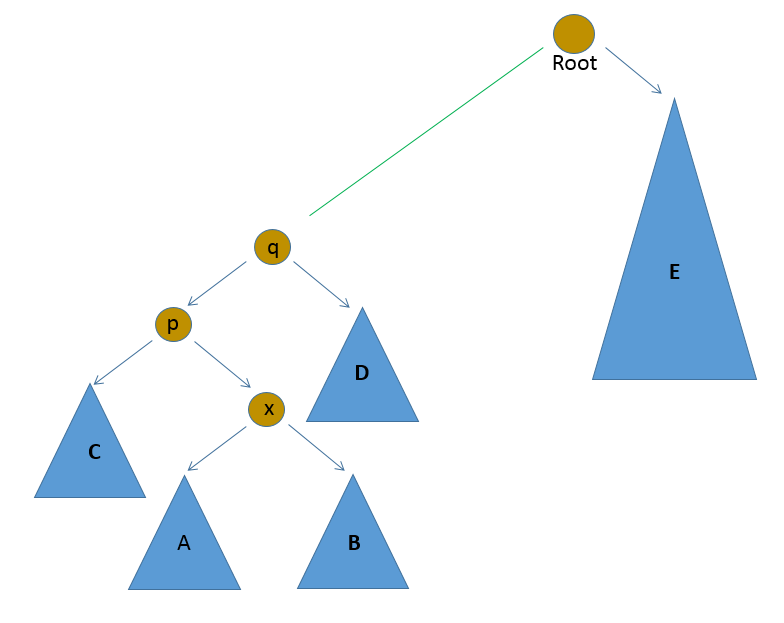
\includegraphics[scale=0.5]{tree.png}
\caption{ Example: Initialise T\_1 as A and T\_2 as B. Now, we go to the parent p, since x is the right child of p, therefore call Special*Union(C,p,T\_1) so that $T\_1 \gets C \cup p \cup T\_1$. Moving further upwards, since p is the left child of q, call Special*Union(T\_2,q,D) so that $T\_2 \gets T\_2 \cup q \cup D$. Similarly, we keep merging untill we reach the root, where we call Special*Union(T\_2,root,E), so that $T\_2 \gets T\_2 \cup root \cup E$ since $x \in left(root)$ }
\label{tree}
\end{center}
\end{figure}


\subsection{Pseudo-Code}
\begin{algorithm}
\caption{Split Red Black Tree}
\label{split}
\begin{algorithmic}[1]
\Procedure{Split(T,x)}{}
\State $cur \gets find(T,x)$   \Comment{\parbox[t]{.5\linewidth}}{Finding x in the given Tree} 
\If{$cur == NULL $}
\State return
\EndIf
\Comment{\parbox[t]{.5\linewidth}}{Initialising $T_1$ and $T_2$} 
\If {$left(cur) \neq NULL $}
\State $T_1 \gets left(cur)$ 
\EndIf
\If {$right(cur) \neq NULL$}
\State $T_2 \gets right(cur)$
\EndIf
\Comment{\parbox[t]{.5\linewidth}}{Moving towards the root} 
\While{$cur \neq NULL$}
\State $cur \gets parent(cur)$
\Comment{\parbox[t]{.5\linewidth}}{Use cur as the key 'y'} 
\If {$val(cur) < x $}
\State $T_1 \gets Special*Union(left(cur),cur,T_1)$ 
\Else
\State $T_2 \gets Special*Union(T_2,cur,right(cur))$
\EndIf
\EndWhile
\EndProcedure
\end{algorithmic}
\end{algorithm}

\subsection{Time Analysis}
Consider the case when we are taking union with respect to $T_1$. Let at any point the height of $T_1$ be $h_i$, and height of left(p) is $h_{i+1}$. Special*Union takes time of $O(h_{i+1}-h_{i})$. Since the height of the RB tree is $O(log(n))$, we will repeat this step $O(log(n))$ times. Thus the complexity will be ,
$$ \sum_{i=1}^{O(log(n))}O(h_{i+1}-h_{i}) = O(log(n)) $$.

\subsection{Space Complexity}
We have taken only $O(1)$ extra space, since we have used only constant number of extra variables.

\section{Connectivity in Real Life}

\subsection{Algorithm}
We first do a DFS traversal from any node of the given graph and generate a rooted tree with no back edge(since the graph is a tree).

\subsubsection{Data Structures Used}
\begin{itemize}
\item An array Label so that, label(v) stores a label which is same for all nodes of the same connected component in the tree(T).
Initially, since the tree is a single connected component,we initialise $label(v)=0$ $ \forall v$ in $T$ . Clearly the size of this array is {\bf n} (number of nodes).

\item An array RootLabel, where RootLabel(i) points to the root of the component with label i for all the nodes in it. The size of this array is also {\bf n}. Initially, RootLabel(0) stores the root of the tree and $RootLabel(i)=NULL$ $\forall i$, $0<i<n$.
\end{itemize}

In addition, we will also keep a variable \textbf{count} which stores the number of connected components currently. 

\subsubsection{Edge Deletion}
After each edge deletion, the number of connected components increases by 1. So, we have to change the label of all the nodes belonging to one of these two newly generated connected components.\\
To reduce the time spent, we find the {\bf smaller component} and change the label for all the nodes in this component.\\

\textbf{Finding Smaller Component} \\
Suppose we have to delete edge(i,j) with i as the parent of j. We have the Label(i) and hence the root of the tree corresponding to this component which is RootLabel(Label(i)), say {\bf a}. \\
After deleting edge(i,j), we will have two connected components with roots being a and j. \\
We will start BFS traversal of the two connected components simultaneously and find which ends first, thus getting the smaller component in time of the order of size of the smaller component.\\

\textbf{Updating label}
\begin{itemize}
\item Assign $Label(v) = count$ where, v is a node of the smaller component.
\item If the smaller component is rooted at j, $then RootLabel(count)=j$, otherwise $then RootLabel(count)=a$ and $then RootLabel(label(a))=j$
\item Increment count.
\end{itemize}

\subsubsection{Answering Query}
If $label(i)=label(j)$, then we say that i and j are connected, otherwise not connected. 

\subsection{Time Analysis}
\subsubsection{Edge Deletion}
Let $T(n)$ be the total time for all edge deletions. We will prove that $T(n)=O(nlog(n))$, using induction. \\
Clearly T(1)= 0, since no query is posible. \\ Assume $T(a) <= ialog(i)+ja+k$ $\forall a$ in $(0,n-1)$.  Now consider,
$$ T(n) = T(a) + T(b) + ma $$  where a is the size of the smaller component after first deletion and $b=n-a$. Then,
$$ T(n) <= ialog(a) + ja+k+iblog(b)+jb+k + ma $$ 
Also , $$ja+k+jb+k <= jn+k$$
Therefore, we can show that ,$$T(n) <= inlog(n)+jn+k$$
if we show that, $$ialog(a)+iblog(b)+k+ma <= inlog(n) $$
or, $$inlog(n)- ialog(a)-iblog(b)-k-ma >=0 $$
\begin{align*}
inlog(n)- ialog(a)-iblog(b)-k-ma &= ialog(n/a)+iblog(n/b)-ma/i-k/i \\
& >= a+ iblog(n/b)-ma/k-k/i\\
& = a(1-m/k) + iblog(n/b)-k/i
\end{align*}
Since $a<=n/2$ and $b>=n/2$, we can find i and k such that the above quantity is always positive. Hence we prove that $T(n)<=inlog(n)+jn+k$ for some i,j and k. Therefore, T(n) takes O(nlog(n)) time.
\subsubsection{Answering Query}
Clearly, it takes $O(1)$ time to answer each query.
\subsection{Space Complexity}
Both the arrays are of size of order n. Thus, total space used is of $O(n)$.

\section{Low Point in DFS traversal}

\subsection{Algorithm}
Given a graph, and arrays S and F, we can find the corresponding DFS tree in O(m+n) time. To compute the array Low\_pt, where Low\_pt(v) stores the Low\_pt of the node v, we do the traversal of the DFS tree two times. First to compute the array Least\_pt (\ref{least}), second to compute the array Low\_pt(\ref{low}).

\subsubsection{Obtaining DFS tree}
We are given arrays S and F. We also know that the values of S for all nodes lies between 0 and 2n-1. So, does the value of F for all the nodes. Thus, we can apply counting sort to sort the arrays S and F in O(2n-1) or O(n) time. Thereafter, using the graph and the sorted S and F arrays, we can compute the DFN values and the DFS tree in O(m+n) time.	

\subsubsection{Least\_pt}
\label{least}
Least\_pt(v) can be defined as the DFN value of the node with the largest DFN value, that is reachable from v, without using any back edge.\\
It can be computed simply using recursion.The Least\_pt of a node is the maximum of the Least\_pt of all it's children(Algorithm \ref{leastAlgo}).

\begin{algorithm}
\caption{Computing Least\_pt}
\label{leastAlgo}
\begin{algorithmic}[1]
\Procedure{Least(v)}{}
\State $max \gets DFN(v) $
\For {all \textbf{children} w of v (if any)} \Comment{\parbox[t]{.5\linewidth}}{Only children, no back edge to be considered} 
\State $temp \gets LEAST(w)$
\If {$temp > max$ }
\State $max \gets temp $
\EndIf
\EndFor
\State $Least\_pt(v) \gets max$
\State return max
\EndProcedure
\end{algorithmic}
\end{algorithm}

\subsubsection{Low\_pt}
\label{low}
As defined in the question, Low\_pt(v) is the DFN value of the node with the largest DFN value, that is reachable from v,using exactly one back edge.\\
Assume that we have the Array Least\_pt already computed. We can compute the Array Low\_pt in a single traversal of the DFS tree. For any node without a back edge, Low\_pt is the maximum of Low\_pt  of all it's children. For a node with a back edge, Low\_pt is simply the maximum of Low\_pt of all it's children and the Least\_pt of the node which is the other end of the back edge.(Algorithm \ref{lowAlgo})

\begin{algorithm}
\caption{Computing Low\_pt}
\label{lowAlgo}
\begin{algorithmic}[1]
\Procedure{Low(v)}{}
\State $max \gets DFN(v)$
\For {all \textbf{children} w of v (if any)} \Comment{\parbox[t]{.5\linewidth}}{Only children, no back edge to be considered} 
\State $temp \gets LOW(w)$
\If {$temp > max$ }
\State $max \gets temp $
\EndIf
\EndFor
\For {all \textbf{u},proper ancestor of v (if any)} 
\State $temp \gets Least\_pt(u)$
\If {$temp > max$ }
\State $max \gets temp $
\EndIf
\EndFor
\State $Low\_pt(v) \gets max$
\State return max
\EndProcedure
\end{algorithmic}
\end{algorithm}

\subsection{Time Analysis}
Computing the DFS tree using the graph, S and F takes O(m+n) time.

\subsubsection{Least\_pt}
Since, we have calculated the array Least\_pt with just one traversal of the DFS tree with 'n' nodes. The time complexity is O(n).

\subsubsection{Low\_pt}
Since, we have calculated the array Low\_pt with just one traversal of the DFS tree with 'n' nodes. The time complexity is O(m+n) again.

\par The total time complexity is therefore,
$$O(m+n) + O(m+n) + O(n) = O(m+n)$$

\subsection{Space Complexity}
Since we have used only two extra arrays other than the DFS tree, the space used is of the order of the input, i.e. O(m+n).

\end{document}


